\section{Synthesis System}
\label{sec:approach}
\autoref{fig:classfy-problem} presents the architecture of \mainname's system, which constructs synthesis derivation trees from which programs are extracted. The construction is achieved in \autoref{alg:synthtree} through a series of queries (\autoref{sec:synthtree-construction-query}), which can be resolved through two approaches corresponding to the dual requirements of our system: code generation (\autoref{sec:query-resolution-lm}) and training data preparation (\autoref{sec:translation}).

The central claim of this section is that constructing a synthesis derivation tree, which is the core of \mainname's framework, is equivalent to constructing an existential type correctness proof. A key insight underlying this equivalence is the isomorphism between type derivation trees and synthesis derivation trees (\autoref{sec:isomorphism}). 
This isomorphism ensures that the constructed synthesis derivation trees maintain the logical flow and dependencies inherent in the type-level reasoning, so that we can construct synthesis derivation trees to represent well-typed programs (\autoref{sec:soundness-completeness}).

\begin{figure}[t]
\centering
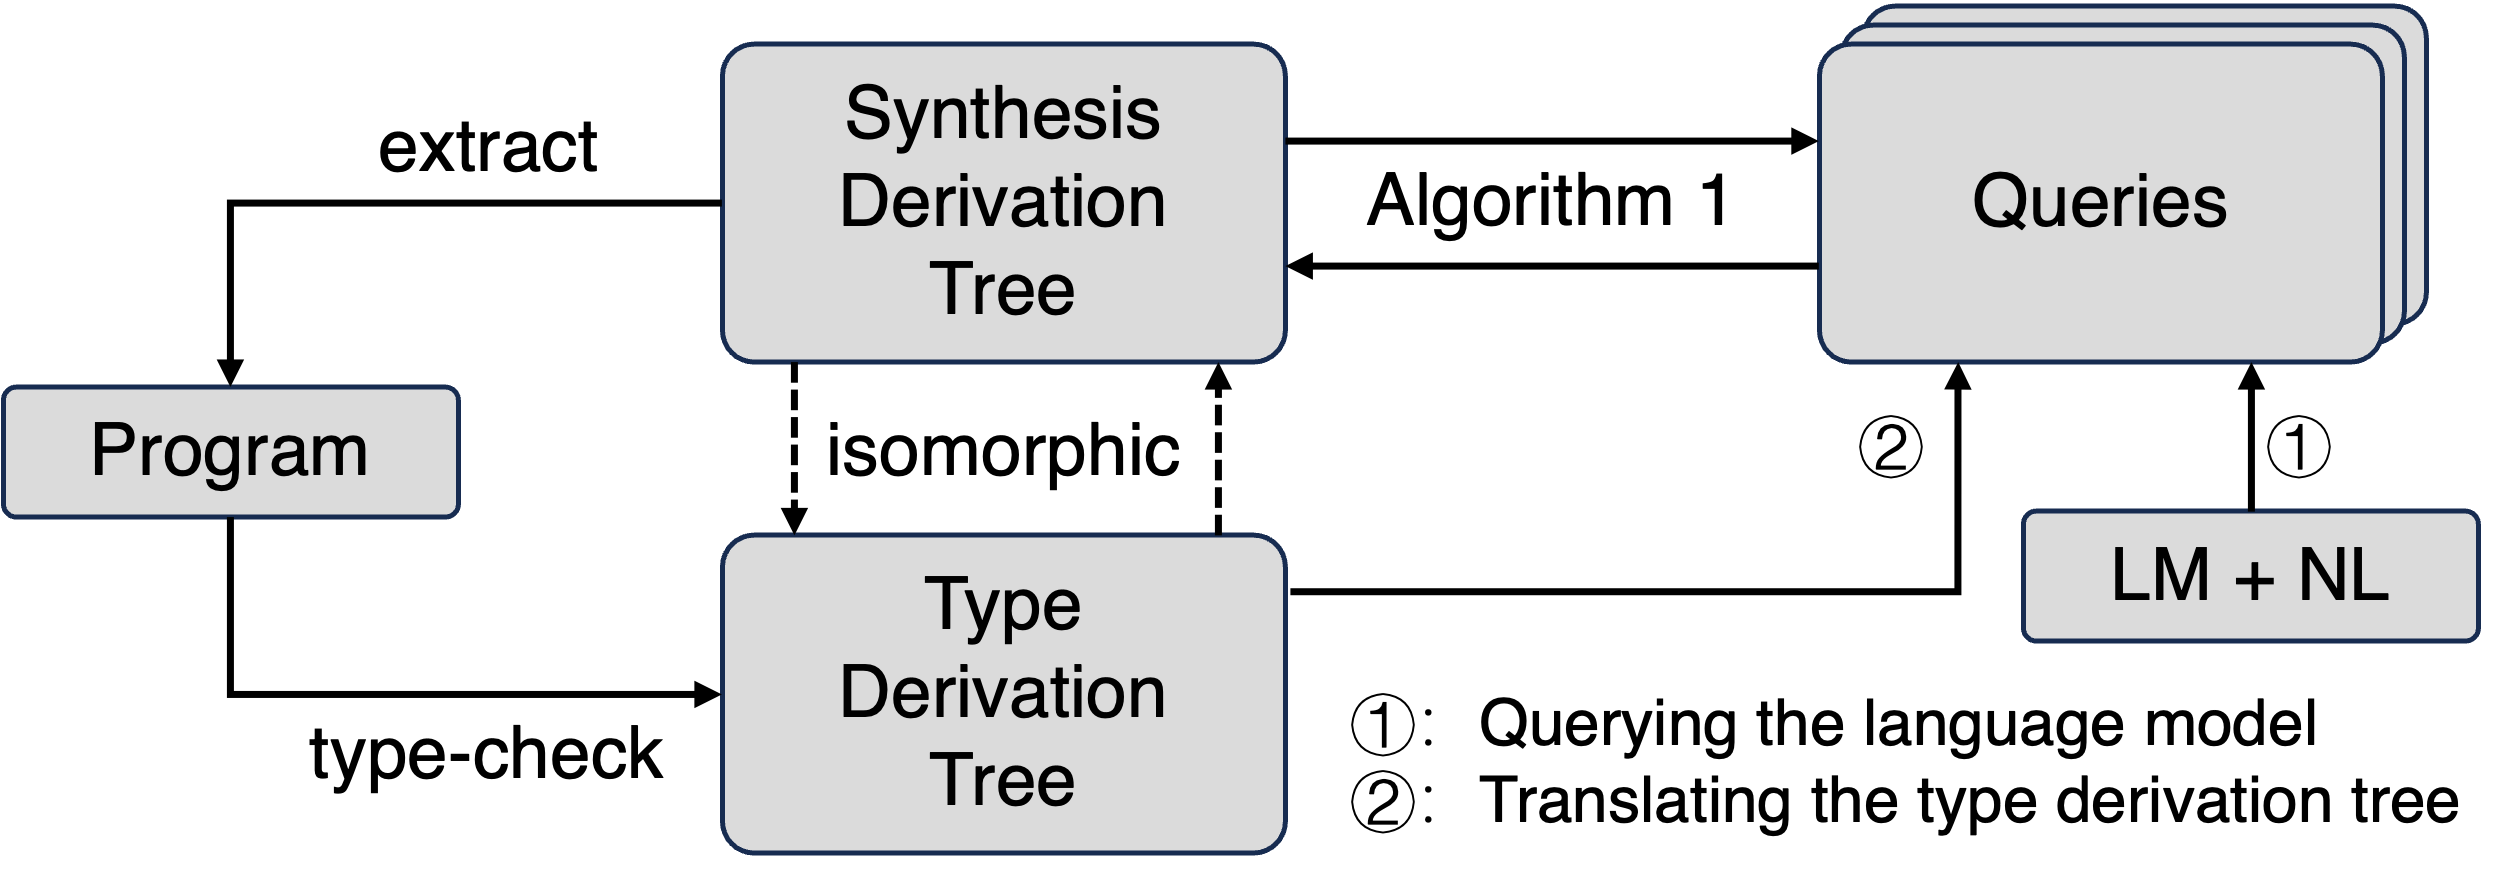
\includegraphics[width=0.75\textwidth]{assets/methods1.png}
\caption{Meta-system architecture of \mainname.}
\label{fig:classfy-problem}
\end{figure}

\subsection{Construction of Synthesis Derivation Trees}
In this subsection, we will first describe the application of synthesis rules (\autoref{sec:synthesis-rule-application}), then introduce the concept of synthesis derivation trees (\autoref{sec:synthesis-derivation-tree}), and finally present the algorithmic construction of synthesis derivation trees, where it is realized by a sequence of query resolutions (\autoref{sec:synthtree-construction-query}).
\subsubsection{Synthesis Rule Application}
\label{sec:synthesis-rule-application}
Each synthesis rule as in \autoref{S-Rule} specifies how to start from a partially instantiated typing judgment $P(\overline{x})$, search for an assignment $\sigma$ to all variables in $\overline{x}$, then derive $P(\sigma(\overline{x}))$ using the corresponding typing rule. This procedure can be detailed as follows:
\begin{enumerate}
    \item \textbf{Unification Step:} First unify the terms in the synthesis goal $P(\overline{x})$ with the terms in the conclusion of the typing rule, yielding the MGU $\sigma$. Once the unification is done, the other terms ($\overline{x}_i$, $\overline{x}_f$, and $\overline{y}$) should also be instantiated with $\sigma$ to match the synthesis goal. Or the unification fails, in which case the synthesis goal is not derivable using this synthesis rule.
    
    % This step ensures that the synthesis goal is aligned with the conclusion of the original typing rule (under certain assignment $\theta$, the resulting $P(\meta{\theta(\skhzc{\overline{x}})})$ can be derived using the original typing rule), or the unification fails, in which case the synthesis goal is not derivable using this synthesis rule.
    
    \item \textbf{Acquisition Step:} Next acquire the assignment for all free variables $\overline{x}_f$ in the synthesis rules (after instantiated by $\sigma$) from external sources. 
    \mainname can infer the term type of each variable to be synthesized based on the definitions of predicates and terms. The generated assignments must conform to the inductively defined syntax described in \autoref{terms-intro}; if any constant or constructor does not match the required term type, the acquisition step fails.
    
    % Free variables can be synthesized either before or after the synthesis of the subgoals. Suppose the synthesis is deferred until after the subgoals. In that case, it is possible to obtain assignments for some variables in $\sigma(\overline{x}_f)$ from among the various $\sigma_i$ (since $\sigma(\overline{x}_f)$ and $\sigma(\overline{x}_i)$ may have shared variables after the unification), postponing the obligation to assign these variables until the last possible moment.
    % However, in practice, it is rare for $\overline{x}_f$ and $\overline{x}_i$ to have no shared variables initially, but to share variables after being instantiated by $\sigma$. If such a situation arises, it is more likely due to the selection of an inappropriate synthesis rule.
    % Therefore, we adopt an eager design approach: synthesizing the assignment $\sigma_0$ for free variables immediately after the unification step. This design encourages the LM to generate the necessary assignment right after choosing the synthesis rule, ensuring semantic coherence throughout the synthesis process.
    
    \item \textbf{Sub-Derivation Steps:} Then, synthesize assignments for all subgoals in sequence. For each subgoal $P_i(\sigma_{i-1}\ldots\sigma_0\sigma(\overline{x}_i)) \leadsto \sigma_i$, begin with an instantiation for variables in $\overline{x}_i$ with the substitutions $\sigma_{i-1}, \ldots, \sigma_0, \sigma$ in previous steps. 
    This refines the subgoal and propagates synthesis information from earlier subgoals. Subsequently, synthesize the assignment $\sigma_i$ for the current subgoal by recursively applying synthesis rules.
    
    \item \textbf{Constraint Checking Step:} After all synthesis subgoals have been solved, \mainname checks whether the constraint $\phi(\overline{y})$  is satisfied under the combined assignment $\sigma_n \ldots \sigma_0 \sigma$. 
    % If the constraint is satisfied, the synthesis rule is considered successfully applied, and we proceed to the final step.
    
    \item \textbf{Assignment Collection Step:} In the final step, \mainname compose all substitutions obtained during synthesis to form $\sigma_c = \sigma_n \ldots \sigma_0 \sigma$, and restrict this assignment to only the variables occurring in $\overline{x}$, yielding the overall assignment $\theta = \sigma_c|_{\mvhzc(\overline{x})}$. 
\end{enumerate}

In steps (3) and (5), we assert without proof that the composed substitution $\sigma_c = \sigma_n \ldots \sigma_0 \sigma$ and the final collected $\theta$ are assignments. Specifically, $\sigma_c$ maps all variables in $\overline{x}$ and $\overline{y}$ to ground terms. This property can be formally established by induction on the structure of the synthesis derivation.

\begin{lemma}
\label{lemma:assignment}
For any successful application of the synthesis rule in \autoref{S-Rule}, the substitution $\sigma_c = \sigma_n \ldots \sigma_0 \sigma$ is an assignment, in the sense that $\forall i$, $\sigma_c(\skhzc{\overline{x}_i})$, $\sigma_c(\skhzc{\overline{x}})$, and $\sigma_c(\skhzc{\overline{y}})$ are all ground terms.
\end{lemma}
\begin{proof}
  %It is proved by induction on the structure of the synthesis derivation.
  The complete proof can be found in Appendix~\ref{sec:appendix-lemma2}.
\end{proof}
% With Lemma~\ref{lemma:assignment}, the successful application of a synthesis rule yields a valid assignment that can concretize the synthesis goal. We will see in the following that we can construct a synthesis derivation tree for the synthesis goal $\welltyped{\skhzc{p}}\leadsto\theta$, which is isomorphic to a type derivation tree of the target program $\theta(\skhzc{p})$.

\subsubsection{Synthesis Derivation Trees}
\label{sec:synthesis-derivation-tree}
To formalize the structure of synthesis derivations, we introduce the concept of synthesis derivation trees in analogy to type derivation trees in type systems. 

A \emph{synthesis derivation tree} is a rooted tree that witnesses the derivability of a synthesis judgment through the application of synthesis rules. More formally, a synthesis derivation tree for a synthesis judgment $P(\skhzc{\overline{t}}) \leadsto \theta$ is a tree where: (1) the root node is labeled with $P(\skhzc{\overline{t}}) \leadsto \theta$; (2) each node is labeled with a synthesis judgment and annotated with both the synthesis rule used and the assignment for its free variables; (3) the children of each internal node correspond to the subgoals of the annotated synthesis rule; (4) for each synthesis rule, all steps including unification, assignment acquisition, subgoals synthesis and constraint checking succeed.

By Lemma~\ref{lemma:assignment}, the existence of a synthesis derivation tree for a synthesis judgment $P(\overline{t}) \leadsto \theta$ guarantees that there is an assignment $\theta$ satisfying the synthesis goal $P(\overline{t})$, that is, $\theta$ maps all variables to ground terms and $P(\sigma(\overline{t}))$ is derivable with respect to typing rules.

\subsubsection{Algorithmic Construction of Synthesis Derivation Trees}
\label{sec:synthtree-construction-query}
The algorithmic construction of synthesis derivation trees is the main focus of \mainname, whether through the interaction with LMs, or via the translation from type derivation trees.
For a synthesis goal of the form $P(\overline{t})$, the task is to synthesize an assignment $\theta$ and construct a synthesis derivation tree with the root node labeled $P(\overline{t}) \leadsto \theta$ by recursively applying synthesis rules as described in \autoref{sec:synthesis-rule-application}.

% The overall construction of the synthesis derivation tree follows a two-phase process:
% \begin{enumerate}
%     \item \textbf{Tree Expansion Phase:} Starting from the synthesis goal $P(\skhzc{\overline{t}})$, we select an appropriate synthesis rule $R$ to apply. We then sequentially perform unification, assignment acquisition (obtaining $\sigma_0$), and recursively synthesize subgoals to expand the synthesis derivation tree.
%     \item \textbf{Assignment Collection Phase:} After synthesizing assignments for all subgoals, we check whether the constraint is satisfied. If so, we can collect the assignment $\theta$ for the original synthesis goal and construct the synthesis derivation tree with a root node labeled $P(\skhzc{\overline{t}}) \leadsto \theta$, annotated with the synthesis rule $R$ and the assignment $\sigma_0$. 
%     If this synthesis goal has a sibling subgoal in another synthesis rule application, the resulting assignment $\theta$ can be used to instantiate the corresponding variables in that sibling subgoal, allowing the propagation of the synthesis information throughout the synthesis derivation tree.
% \end{enumerate}

\begin{algorithm}[tb]
  \caption{Synthesis Derivation Tree Construction}
  \label{alg:synthtree}
  \KwIn{A synthesis goal $P(\skhzc{\overline{t}})$}
  \KwOut{A synthesis derivation tree $T$ whose root node is labeled $P(\skhzc{\overline{t}}) \leadsto \theta$}
  \SetKwFunction{GenSynthTree}{GenSynthTree}
  \SetKwProg{Fn}{Function}{:}{}
  
  \Fn{\GenSynthTree{$P(\overline{t})$}}{
    Select a synthesis rule $R$ with conclusion $P(\overline{x}) \leadsto \ldots$
    \tcp*{Suppose $R$ is as \autoref{S-Rule}}
    
    Instantiate $\overline{x}$ with $\overline{t}$ in $R$\;
    $\sigma \gets$ MGU from the unification step of $R$\;
    \lIf{$\sigma = \bot$}{\Return{$\bot$}} 

    $\sigma_0 \gets \func{AcquireFreeVariableAssignment}(\sigma(\overline{x}_f))$\;
    \lIf{$\sigma_0 = \bot$}{\Return{$\bot$}}
    
    \ForEach{\textnormal{subgoal} $P_i(\sigma_{i-1} \ldots \sigma_1 \sigma(\overline{x}_i))$ \textnormal{of} $R$}
    {
        $T_i \gets \GenSynthTree{ $P_i(\sigma_{i-1} \ldots \sigma_1 \sigma(\overline{x}_i))$} $\;
        \lIf{$T_i = \bot$}{\Return{$\bot$}}
        $\sigma_i \gets$ assignment from the root node of $T_i$\;
    }
    
    \lIf{$\phi(\sigma_n \ldots \sigma_0 \sigma(\overline{y})) = \bot$}{\Return{$\bot$}}
    $\theta \gets \sigma_n \ldots \sigma_0 \sigma|_{\mvhzc(\overline{t})}$\;
    \Return{$\func{MakeTreeNode}(P(\overline{t}) \leadsto \theta, R, \sigma_0, T_1, \ldots, T_n)$}
}
\end{algorithm}

This process is detailed in \autoref{alg:synthtree}. In this algorithm, only two functions act as black boxes: the selection of synthesis rules and the acquisition of assignments for free variables. Both can be viewed as query problems. Synthesis rule selection is a single-step query that chooses one rule from a finite set of candidates, while assignment acquisition is a multi-step query that constructs a ground term for each free variable using a finite set of constructors and constants.

Consequently, our approach reduces the synthesis problem to finding appropriate solvers for these two specific query problems. This makes our framework more general and modular, as the extracted query resolution problems can be implemented independently. 
Moreover, the in-time checking mechanisms (unification and constraint verification, etc.) in \autoref{alg:synthtree} significantly restrict the search space compared to naive enumeration-based approaches. 
%This structured decomposition not only simplifies implementation but also enables leveraging existing LMs tailored for query-based tasks to address each component effectively.

\subsection{Query Resolution}
\autoref{fig:classfy-problem} illustrates how query resolution serves as a central mechanism in constructing a synthesis derivation tree. Queries should be resolved to determine which synthesis rule to apply and how to instantiate variables. In the following, we present two complementary approaches for query resolution: employing LMs to make decisions during code generation (\autoref{sec:query-resolution-lm}), and translating type derivation trees to prepare supervised training data (\autoref{sec:translation}).

\subsubsection{Query Resolution using LMs}
\label{sec:query-resolution-lm}
In the code generation scenario, both query resolution functions are delegated to the LM, which, given the natural language input, acts as a decision-making component for synthesis rule selection and variable assignment.

\begin{itemize}
  \item \textbf{Selection of synthesis rules:} Given the natural language description, the current partially constructed synthesis derivation tree, and the synthesis goal, the LM is expected to choose a specific synthesis rule from the available rule set.
  
  \item \textbf{Assignment of free variables:} After a synthesis rule is selected and unification is performed, the LM is required to generate a sequence of constructors and constants, constructing ground terms for assigning free variables. 
  % These assignments fill in the concrete details (such as variable names, constants, or operators) that are not determined by the rule structure alone.
\end{itemize}

LM prediction is performed in a contextually aware manner, conditioned on multiple sources of information: (1) the natural language describing the desired program behavior; (2) the current synthesis derivation tree, which encodes both the ongoing synthesis process and the type derivation process via the isomorphism between type and synthesis derivation trees; and (3) the synthesis goal $P(\overline{t})$, which includes already synthesized program fragments and the current typing context.

The LM leverages its learned type-reasoning ability to generate the most appropriate synthesis rule and corresponding variable assignments by jointly reasoning about the semantic intentions conveyed by the natural language and the structural requirements encoded in the derivation tree. 
% More detailed information about how the LM receives the information and makes decisions can be found in Section~\ref{sec:implementation}. 

\subsubsection{Query Resolution through Type Derivation Tree Translation}
\label{sec:translation}
Beyond the code generation scenario in which natural language serves as input, \mainname requires curated training data to teach the LM how to interpret and solve synthesis queries. 
We generate such queries by translating existing type derivation trees of target programs, which involves recording the contextual information and the ground truth decision at each step of synthesis rule application.

% By capturing these query-answer pairs throughout the synthesis process, we can provide the LM with supervised training examples that demonstrate how to make appropriate synthesis rule selections and variable assignments at each decision point.
The translation is performed by traversing the type derivation tree. When we visit its root node, we begin constructing the synthesis derivation tree from the root node too. 
For the $i$-th child labeled $P_i(\overline{x}_i)$ of the current node $n_1$ in the type derivation tree, upon entering its corresponding subtree, we construct the synthesis derivation tree for the $i$-th subgoal $P_i(\sigma_{i-1} \ldots \sigma_0 \sigma(\overline{x}_i))$ too.

When we return to the node $n_1$, the synthesis derivation trees for all subgoals have been constructed, allowing us to build node $n_2$ in the synthesis derivation tree. At every stage of the synthesis process, there is a node in the type derivation tree corresponding to the current synthesis goal.

\begin{itemize}
  \item \textbf{Selection of synthesis rules:}  
  Assume the node $n_1$ is labeled with a typing judgment $P(\overline{x}_c)$, annotated with a typing rule $R$, and the synthesis goal is $P(\overline{x})$. Following the procedure in \autoref{sec:meta-translation}, we translate $R$ into a synthesis rule $R'$, which is the synthesis rule to be applied.
  
  \item \textbf{Assignment of free variables:}  
    Assume the typing rule $R$ has the form in \autoref{T-Rule}, and the synthesis rule $R'$ has the form in \autoref{S-Rule}. 
    Then $P(\overline{x}_c)$ is the concretization of both the conclusion $P(\overline{x}_0)$ of the typing rule and the synthesis goal $P(\overline{x})$ (can be proved later). 
    Thus, $\overline{x}_0$ and $\overline{x}$ are unifiable, and the MGU $\sigma$ makes $\sigma(\overline{x}) = \sigma(\overline{x}_0)$ unifiable with $\overline{x}_c$. Therefore, there exists an assignment $\theta'$ such that $\theta'\sigma(\overline{x}_0) = \overline{x}_c$ and $\theta'$ covers $\mvhzc(\sigma(\overline{x}_0))$. Since $\mvhzc(\overline{x}_f) \subseteq \mvhzc(\overline{x}_0)$, we have $\mvhzc(\sigma(\overline{x}_f)) \subseteq \mvhzc(\sigma(\overline{x}_0))$, so $\theta'$ can also cover $\mvhzc(\sigma(\overline{x}_f))$. Let $\sigma_0 = \theta'|_{\mvhzc(\sigma(\overline{x}_f))}$ be the assignment for the free variables in the synthesis rule.
\end{itemize}

Since the translation begins from a valid type derivation tree, it is guaranteed to produce a valid synthesis derivation tree. In particular, the unification, assignment acquisition, and constraint checking steps will always succeed, and the synthesized assignment $\theta$ concretizes the original synthesis goal $P(\overline{x})$ to the typing judgment $P(\overline{x}_c)$ labeled at the root of the type derivation tree.

\begin{lemma}
\label{lemma:translation}
Let $T_1$ be a type derivation tree whose root node is labeled $P(\overline{x}_c)$, annotated with typing rule $R$, and $T_2$ be the translated synthesis derivation tree, whose root node is labeled $P(\overline{x}) \leadsto \theta$.
%where $\theta$ is synthesized by \autoref{alg:synthtree}.
If $\,\overline{x}$ is unifiable with $\overline{x}_c$, then in the application of the synthesis rule $R'$ that derives $P(\overline{x}) \leadsto \theta$, (1) the unification step, (2) the acquisition step, and (3) the constraint checking step will succeed, and (4) the synthesized assignment $\theta$ concretizes $P(\overline{x})$ to $P(\theta(\overline{x}))$, which is equal to $P(\overline{x}_c)$.
\end{lemma}
\begin{proof}
  %It is proved by induction on the structure of the type derivation tree $T_1$.
  The complete proof can be found in the Appendix~\ref{sec:appendix-lemma3}.
\end{proof}

With Lemma~\ref{lemma:translation}, we can conclude that given a type derivation tree $T_1$ whose root node is labeled $\welltyped{p_c}$, we can start from the synthesis goal $\welltyped{\sk{p}}$, where $\sk{p}$ is a variable representing the program to be synthesized, and construct a synthesis derivation tree $T_2$ by translating from $T_1$ such that the root node of $T_2$ is labeled $\welltyped{\sk{p}} \leadsto \theta$, where $\theta(\sk{p}) = p_c$.

\subsection{Isomorphism between Type Derivation Trees and Synthesis Derivation Trees}
\label{sec:isomorphism}
Since every synthesis rule is translated from a typing rule, and every synthesis subgoal in the synthesis rule corresponds to a premise in the typing rule, we can establish an isomorphism between synthesis derivation trees and type derivation trees.

\paragraph{Isomorphism of Derivation Trees}
A type derivation tree $T_1 = (V_1, r_1)$ (with node set $V_1$ and root $r_1$) and a synthesis derivation tree $T_2 = (V_2, r_2)$ are \emph{isomorphic} if there exists a bijection $\varphi: V_1 \to V_2$ satisfying the following conditions:
\begin{enumerate}
    \item Root Correspondence: $\varphi(r_1) = r_2$
    \item Child Order Preservation: For $v \in V_1$, if $\mathsf{children}_{T_1}(v) = [v_1, \ldots, v_k]$, where $\mathsf{children}_{T}(v)$ denotes the ordered list of $v$'s children in tree $T$, then $\mathsf{children}_{T_2}(\varphi(v)) = [\varphi(v_1), \ldots, \varphi(v_k)]$
    \item Label/Annotation Correspondence: For every $v \in V_1$ labeled with typing judgment $P(\overline{t}_c)$ and a typing rule, $\varphi(v)$ is labeled with synthesis judgment $P(\skhzc{\overline{t}}) \leadsto \theta$, annotated with the corresponding synthesis rule and assignment, where $\theta(\skhzc{\overline{t}}) = \overline{t}_c$
\end{enumerate}
We write $T_1 \cong T_2$ to denote that $T_1$ and $T_2$ are isomorphic, representing the same logical structure but in different forms.
%
The translation procedure described in \autoref{sec:translation} provides a systematic way to construct an isomorphic synthesis derivation tree from any given type derivation tree. During this process, for each node $n_1$ in the type derivation tree, we define the correspondence $\varphi(n_1) = n_2$, where $n_2$ is the node constructed by translating $n_1$. It is straightforward to verify that this bijection preserves the root nodes and the order of children, and, by Lemma~\ref{lemma:translation}, also preserves the correspondence of labels and annotations. Thus, $T_1 \cong T_2$, as captured by the following lemma.

\begin{lemma}
\label{lemma:isomorphism1}
For any type derivation tree $T_1$, there exists a synthesis derivation tree $T_2$, $T_1 \cong T_2$.
\end{lemma}

Conversely, we can construct a type derivation tree $T_1$ from a given synthesis derivation tree $T_2$, also preserving isomorphism. The construction is straightforward: we traverse $T_2$, and for each node labeled with the synthesis goal $P(\overline{t}) \leadsto \theta$, we create a corresponding node labeled with the typing judgment $P(\theta(\overline{t}))$ and annotate it with the appropriate typing rule. Similar to Lemma~\ref{lemma:translation}, we can inductively show that the resulting $T_1$ is a type derivation tree, and that the bijection between $T_1$ and $T_2$ ensures the isomorphism $T_1 \cong T_2$.

\begin{lemma}
\label{lemma:isomorphism2}
For any synthesis derivation tree $T_2$, there exists a type derivation tree $T_1$, $T_1 \cong T_2$.
\end{lemma}
\begin{proof}
  The complete proof can be found in the Appendix~\ref{sec:appendix-lemma4}.
\end{proof}

\subsection{Soundness and Completeness}
\label{sec:soundness-completeness}
We have established an isomorphism between type derivation trees (type correctness proofs) and synthesis derivation trees (existential type correctness proofs). 
%As a result, synthesis derivation trees both collect assignments to the variables in the synthesis goals and represent the type derivation process for the synthesized programs. 
Under the isomorphism, \mainname ensures that well-typed programs can always be \emph{extracted} from synthesis derivation trees, rather than relying on direct program synthesis without reference to their type correctness proofs.

% \paragraph{Extracting Well-Typed Programs}
The notions of ``extract'' and ``well-typed'' can be formally defined in the context of derivation trees. 
Given a synthesis derivation tree with root node labeled $\welltyped{\sk{p}} \leadsto \theta$, the extracted program is $\theta(\sk{p})$. And a program $p_c$ is said to be well-typed if there exists a type derivation tree (type correctness proof) whose root node is labeled $\welltyped{p_c}$.

\begin{theorem}[Soundness]
Any program extracted from a synthesis derivation tree $T$ is well-typed.
\end{theorem}
\begin{proof}
Suppose the root node of $T$ is labeled $\welltyped{\sk{p}} \leadsto \theta$. By Lemma~\ref{lemma:isomorphism2}, there is a type derivation tree $T'$ such that $T \cong T'$. The root node of $T'$ is labeled $\welltyped{p_c}$, where $p_c = \theta(\sk{p})$ is the program extracted from $T$. By the definition of well-typed programs, $p_c$ is well-typed.
\end{proof}

\begin{theorem}[Completeness]
For any well-typed program $p_c$, there exists a synthesis derivation tree such that the program extracted from it is $p_c$.
\end{theorem}
\begin{proof}
There exists a type derivation tree $T_1$ whose root node is labeled $\welltyped{p_c}$. By Lemma~\ref{lemma:isomorphism1}, there exists a synthesis derivation tree $T_2$ such that $T_1 \cong T_2$. The root node of $T_2$ is labeled $\welltyped{\sk{p}} \leadsto \theta$, where $\theta(\sk{p}) = p_c$. Thus, the program extracted from $T_2$ is $p_c$.
\end{proof}

\begin{corollary}
The synthesis derivation tree $T$ guaranteed by the completeness theorem is precisely the tree obtained through the translation process described in \autoref{sec:translation}.
\end{corollary}

The soundness and completeness theorems ensure the correspondence between well-typed programs and synthesis derivation trees. This correspondence works in both directions: every well-typed program can be represented as a synthesis derivation tree (completeness), and every synthesis derivation tree yields a well-typed program (soundness). Together, these results confirm that constructing a synthesis derivation tree is equivalent to constructing an existential type correctness proof: the isomorphism with type derivation trees provides the proof structure, while the synthesized assignment provides the witness (the program) that makes the existential statement $\exists p.\; \welltyped{p}$ hold.